 \chapter{System- und Hardware-Entwurf}
 \label{cha:hardware}
 
 Nach der vollständigen Definition der Systemanforderungen begann gemäß dem Wasserfall-Modell die Entwurfsphase. In diesem Schritt wurde die abstrakte Problemlösung in eine konkrete Systemarchitektur und eine physikalische Hardware-Auslegung überführt. Ein besonderer Fokus lag dabei auf der Kosteneffizienz sowie der zuverlässigen Ansteuerung der Sensorik und Aktorik.
 
 \section{Systemarchitektur}
 Die Systemarchitektur bildet das Herzstück des Hardware-Designs und zeigt das Zusammenspiel aller verwendeten Komponenten. Die logische und elektrische Verknüpfung der Bauteile mit dem Mikrocontroller ist in Abbildung \ref{fig:systemarchitektur} dargestellt.
 
 \begin{figure}[h]
 	\centering
 	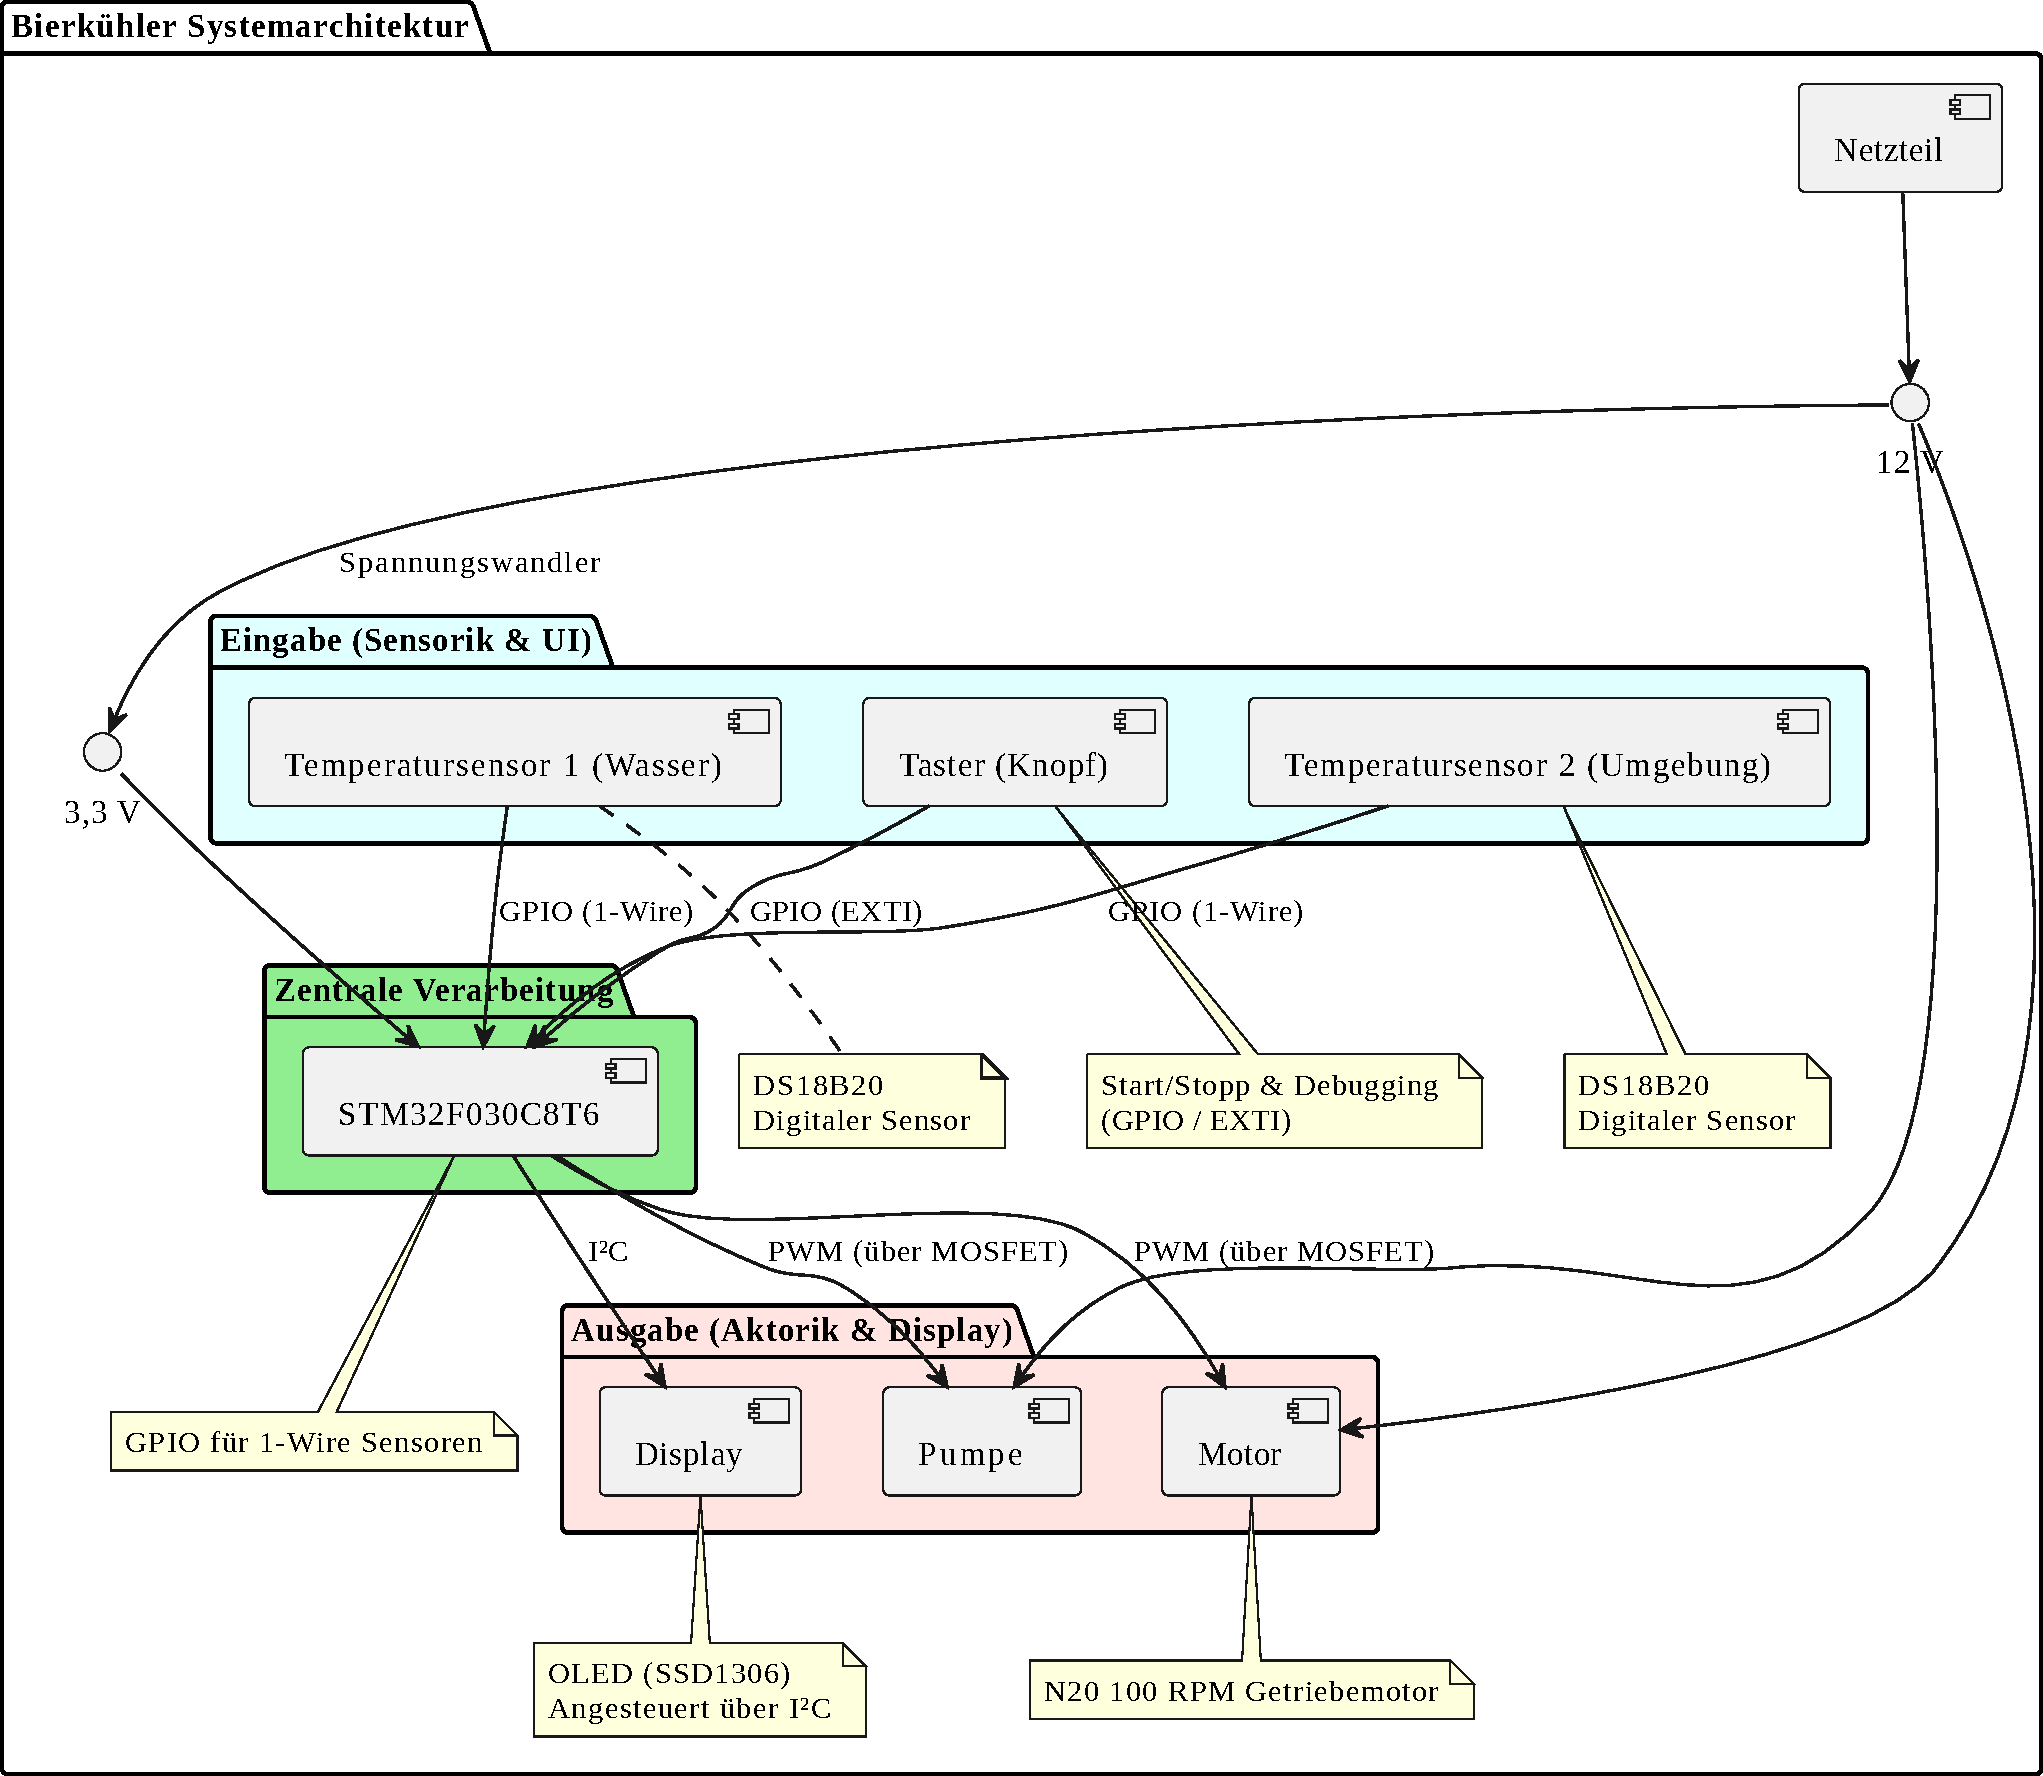
\includegraphics[width=\textwidth]{images/systemarchitektur.pdf} 
 	\caption{Systemarchitektur des Bierkühlers (Hardware-Ebene)}
 	\label{fig:systemarchitektur}
 \end{figure}
 
 Das System ist grob in drei funktionale Blöcke unterteilt: Die Eingabe (Sensorik und Nutzer-Interface), die zentrale Verarbeitungseinheit (MCU) und die Ausgabe (Aktorik und Display).
 
 \section{Komponentenauswahl und Technical Trades}
 Im Rahmen des Hardware-Designs wurden verschiedene Komponenten evaluiert und \textit{Technical Trades} (technische Abwägungen) durchgeführt, um einen Kompromiss aus Kosten, Leistungsfähigkeit und Entwicklungsaufwand zu finden.
 
 \subsection{Mikrocontroller und Spannungsversorgung}
 Als zentrale Steuereinheit wurde der \textbf{STM32F030C8T6} gewählt. Dieser Mikrocontroller bietet für das Projekt die ideale Balance aus geringen Beschaffungskosten und ausreichender Peripherieausstattung (mehrere ADC-Kanäle, Hardware-Timer für PWM und I²C-Schnittstellen) \cite{stm32f030_datasheet}. 
 
 Das System arbeitet mit zwei Spannungsdomänen:
 \begin{itemize}
 	\item \textbf{12V-Kreis:} Die Aktorik (Motor für die Flaschenrotation und Wasserpumpe) benötigt eine höhere Leistung, die direkt vom Netzteil bereitgestellt wird.
 	\item \textbf{3,3V-Kreis:} Ein Spannungswandler (Step-Down) transformiert die 12V auf 3,3V, um den Mikrocontroller, das Display und die Sensoren stabil zu versorgen.
 \end{itemize}
 
 \subsection{Sensorik (Eingabe)}
 Für die Temperaturüberwachung (vgl. Anforderung ID-0008) kommen zwei digitale Temperatursensoren vom Typ \textbf{DS18B20} zum Einsatz. Ein Sensor überwacht die Wassertemperatur im Kühlbehälter, der zweite die Umgebungstemperatur. Im Gegensatz zu analogen Sensoren werden diese direkt über das 1-Wire-Protokoll an handelsüblichen GPIO-Pins des STM32 ausgelesen \cite{ds18b20_datasheet}, was den internen ADC (Analog-to-Digital Converter) entlastet und die Anfälligkeit für Signalrauschen minimiert.
 
 Im Rahmen eines iterativen Scope-Managements wurde aus zeitlichen Restriktionen auf den ursprünglich angedachten Rotary Encoder verzichtet. Für die Benutzereingabe (ID-0010) wird stattdessen ein einzelner \textbf{Taster (Knopf)} verwendet, der als zentrales Steuerelement (Start/Stopp-Logik der Kühlung sowie für Debugging-Zwecke) fungiert. Dieser ist an einen digitalen GPIO-Pin angebunden und nutzt externe Interrupts (EXTI). Dies gewährleistet, dass der Mikrocontroller verzögerungsfrei auf das Eingabesignal reagiert, ohne die CPU durch ständiges Polling zu belasten.
 
 \subsection{Aktorik (Ausgabe)}
 Die Ausgabe-Hardware stellte den kritischsten Punkt im Designprozess dar. Wie bereits in der Anforderungsanalyse beschrieben, wurde hier ein technischer Trade-off vollzogen: Anstelle eines elektromechanischen Relais übernehmen \textbf{Leistungs-MOSFETs} das Schalten der 12V-Komponenten. Hierzu zählen die Wasserpumpe sowie ein \textbf{N20 100RPM Getriebemotor}, der für die kontinuierliche Rotation der Flasche zuständig ist.
 
 Das Gate dieser Leistungstransistoren ist direkt mit den entsprechenden GPIO-Pins des STM32 verbunden. Durch die Ausgabe eines Pulsweitenmodulations-Signals (PWM) kann die zugeführte Leistung für Motor und Pumpe stufenlos und nahezu leistungslos geregelt werden. Dies schützt den Mikrocontroller vor elektrischer Überlastung und erfüllt gleichzeitig die Performance-Anforderung (ID-0003), die Rotationsgeschwindigkeit präzise anzupassen, um das Bier vor übermäßigem Schäumen zu bewahren.
 
 \subsection{User Interface}
 Zur Visualisierung des Systemstatus (aktuelle Temperaturen und Kühlstatus) wurde ein \textbf{OLED-Display} (Controller SSD1306) implementiert. Um wertvolle GPIO-Pins am Mikrocontroller zu sparen und das Platinen-Layout einfach zu halten, wird das Display über den seriellen \textbf{I²C-Bus} (Inter-Integrated Circuit) angesteuert. Hierfür werden lediglich zwei Leitungen (SDA für Daten und SCL für den Takt) benötigt.